\subsection{Атаки по сторонним каналам}
\begin{frame}{\insertsubsection}

  \begin{figure}[h]
    \center%
    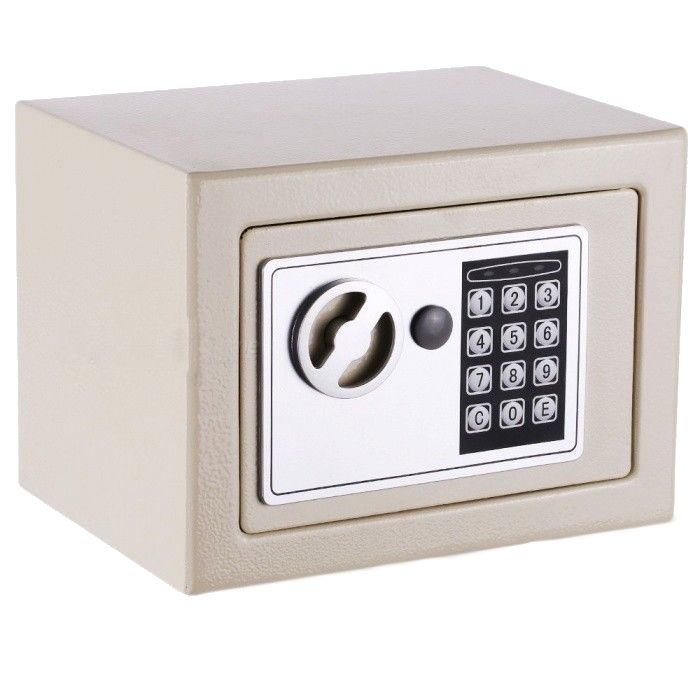
\includegraphics[height = .8\textheight]{safe_guard}
    \caption{Пример цели для атаки по сторонним каналам}
  \end{figure}

  \note{

    Идея атак по сторонним каналам \textbf{весьма стара}, ещё в 1980-х годах
    было о них известно. Но широкое распространение данный вид атак получил
    только после публикации \textbf{Пола Кохера в 1996 году}.

    Самый примитивный пример атаки по сторонним каналам --- \textbf{определение
      нажатых кнопок сейфа по звуку} при введении секретного кода.

    Такого рода атаки обычно основываются на вычислении изменений в окружающей
    среде, например, изменения в \textbf{потреблении тока устройством,
      электромагнитном излучении, температуре, по издаваемым акустическим
      сигналам, по времени,} затрачиваемому на выполнение тех или иных операций
    и другие.

  }
\end{frame}

\subsection{Атаки на микроархитектуру}
\begin{frame}[fragile]{\insertsubsection}


  \begin{columns}
    \begin{column}{.3\textwidth}
      \begin{minted}[]{nasm}
        code1a:
          mov (X), %eax
          mov (Y), %ebx
          clflush (X)
          clflush (Y)
          jmp code1a
      \end{minted}
    \end{column}

    \begin{tikzpicture}
      \draw[line width = 3pt, -{Stealth[length = 1cm]}] (0,0) -- (3,0);
    \end{tikzpicture}

    \begin{column}{.5\textwidth}
      \begin{figure}[h]
        \center%
        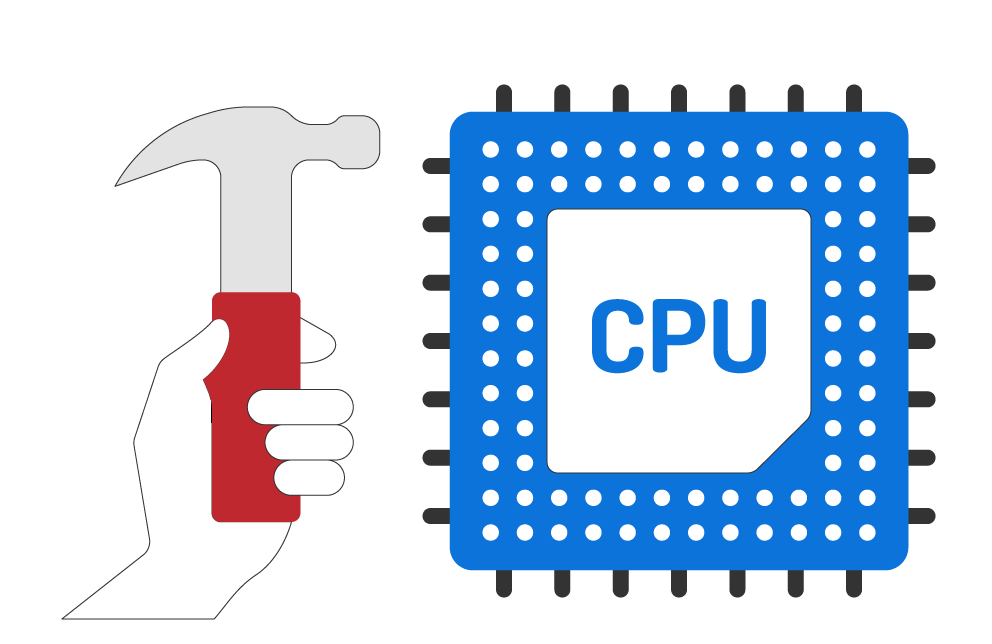
\includegraphics[width = .6\textwidth]{cpu_break}
        \caption{При эксплуатации аппаратных дефектов есть шанс нанести физические
          повреждения}
      \end{figure}
    \end{column}
  \end{columns}

  \note{

    Атаки по сторонним каналам на микроархитектуру, основанные на использовании
    программного обеспечения, как правило, даже \textbf{не требуют физического
      доступа} к вычислительному устройству.

    Также существуют атаки, \textbf{основанные на дефектах микроархитектуры},
    например, ошибки, происходящие \textbf{во время оптимизации}.

    Атаки на микроархитектуру, которые используют аппаратные дефекты,
    \textbf{сложно воссоздать на практике,}. Примеров таких атак не много, но
    все они широко известны, это например, \textbf{Rowhammer атака,} которая, в
    случае успешно разработанного потока инструкций, может дестабилизировать
    работу процессора и даже нанести \textbf{неисправимые физические
      повреждения,} если атака будет проводиться в течении нескольких недель.

    \textbf{Все уязвимости можно найти, просто почитав} главу оптимизаций в
    \textbf{спецификации процессора}, даже на Wiki есть раздел про оптимизацию
    работы CPU, в которой перечислены все элементы, в которых были найдены
    уязвимости.

  }

\end{frame}
